\documentclass[tikz]{standalone}
% \usepackage{tikz} % already loaded by the documentclass


\begin{document}
%%| filename: hidden-layer-example
%%| caption: Multi-Couches
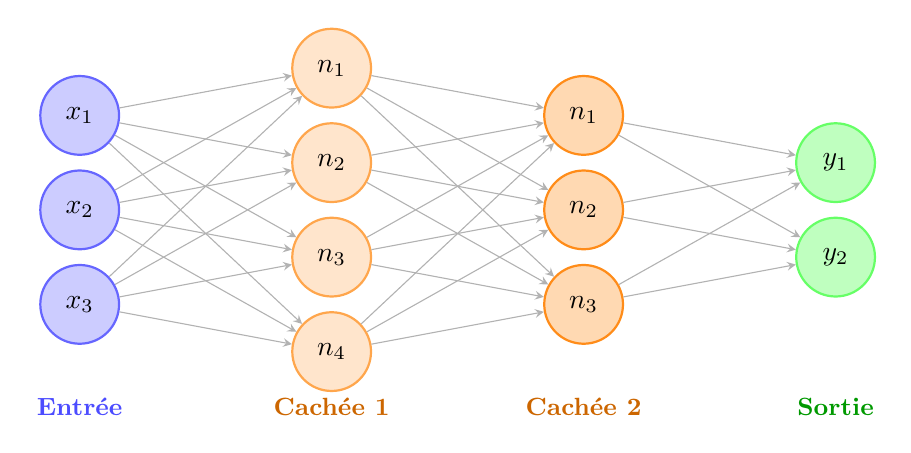
\begin{tikzpicture}[
    input neuron/.style={
        circle,
        draw=blue!60,
        fill=blue!20,
        thick,
        minimum size=1cm,
        inner sep=0pt
    },
    hidden1 neuron/.style={
        circle,
        draw=orange!70,
        fill=orange!20,
        thick,
        minimum size=1cm,
        inner sep=0pt
    },
    hidden2 neuron/.style={
        circle,
        draw=orange!90,
        fill=orange!30,
        thick,
        minimum size=1cm,
        inner sep=0pt
    },
    output neuron/.style={
        circle,
        draw=green!60,
        fill=green!25,
        thick,
        minimum size=1cm,
        inner sep=0pt
    },
    connection/.style={
        ->,
        >=stealth,
        gray!60,
        line width=0.4pt
    }
]

\def\layersep{3.2}
\def\nodesep{1.2}

%% --- Couche d'entrée (3 neurones) ---
\node[input neuron] (X1) at (0, 1*\nodesep) {$x_1$};
\node[input neuron] (X2) at (0, 0)          {$x_2$};
\node[input neuron] (X3) at (0, -1*\nodesep) {$x_3$};

%% --- Couche cachée 1 (4 neurones) ---
\node[hidden1 neuron] (H11) at (\layersep,  1.5*\nodesep) {$n_1$};
\node[hidden1 neuron] (H12) at (\layersep,  0.5*\nodesep) {$n_2$};
\node[hidden1 neuron] (H13) at (\layersep, -0.5*\nodesep) {$n_3$};
\node[hidden1 neuron] (H14) at (\layersep, -1.5*\nodesep) {$n_4$};

%% --- Couche cachée 2 (3 neurones) ---
\node[hidden2 neuron] (H21) at (2*\layersep,  1*\nodesep) {$n_1$};
\node[hidden2 neuron] (H22) at (2*\layersep,  0)          {$n_2$};
\node[hidden2 neuron] (H23) at (2*\layersep, -1*\nodesep) {$n_3$};

%% --- Couche de sortie (2 neurones) ---
\node[output neuron] (Y1) at (3*\layersep,  0.5*\nodesep) {$y_1$};
\node[output neuron] (Y2) at (3*\layersep, -0.5*\nodesep) {$y_2$};

%% --- Connexions entrée -> cachée 1 (toutes) ---
\foreach \src in {1,2,3} {
    \foreach \dst in {1,2,3,4} {
        \draw[connection] (X\src) -- (H1\dst);
    }
}

%% --- Connexions cachée 1 -> cachée 2 (toutes) ---
\foreach \src in {1,2,3,4} {
    \foreach \dst in {1,2,3} {
        \draw[connection] (H1\src) -- (H2\dst);
    }
}

%% --- Connexions cachée 2 -> sortie (toutes) ---
\foreach \src in {1,2,3} {
    \foreach \dst in {1,2} {
        \draw[connection] (H2\src) -- (Y\dst);
    }
}

%% --- Étiquettes des couches ---
\node[font=\small\bfseries, text=blue!70]         at (0,          -2.5) {Entrée};
\node[font=\small\bfseries, text=orange!80!black] at (\layersep,  -2.5) {Cachée 1};
\node[font=\small\bfseries, text=orange!80!black] at (2*\layersep,-2.5) {Cachée 2};
\node[font=\small\bfseries, text=green!60!black]  at (3*\layersep,-2.5) {Sortie};

\end{tikzpicture}
\end{document}
      